\section{Methodology}
\label{sec:method}

Describe \methodname{}. Introduce notation, define the problem formally, and then
present your approach. Number important equations so you can reference them, e.g.
\cref{eq:objective}:
\begin{equation}
    \mathcal{L}(\theta) = \frac{1}{N} \sum_{i=1}^{N}
        \ell\big(f_\theta(x_i),\, y_i\big).
    \label{eq:objective}
\end{equation}

\subsection{Component One}
\label{subsec:component-one}
Explain the first component of your method. Figures live under \texttt{figures/}
and are included with \texttt{\textbackslash includegraphics}. \cref{fig:overview}
shows a single-image figure.

\begin{figure}[t]
    \centering
    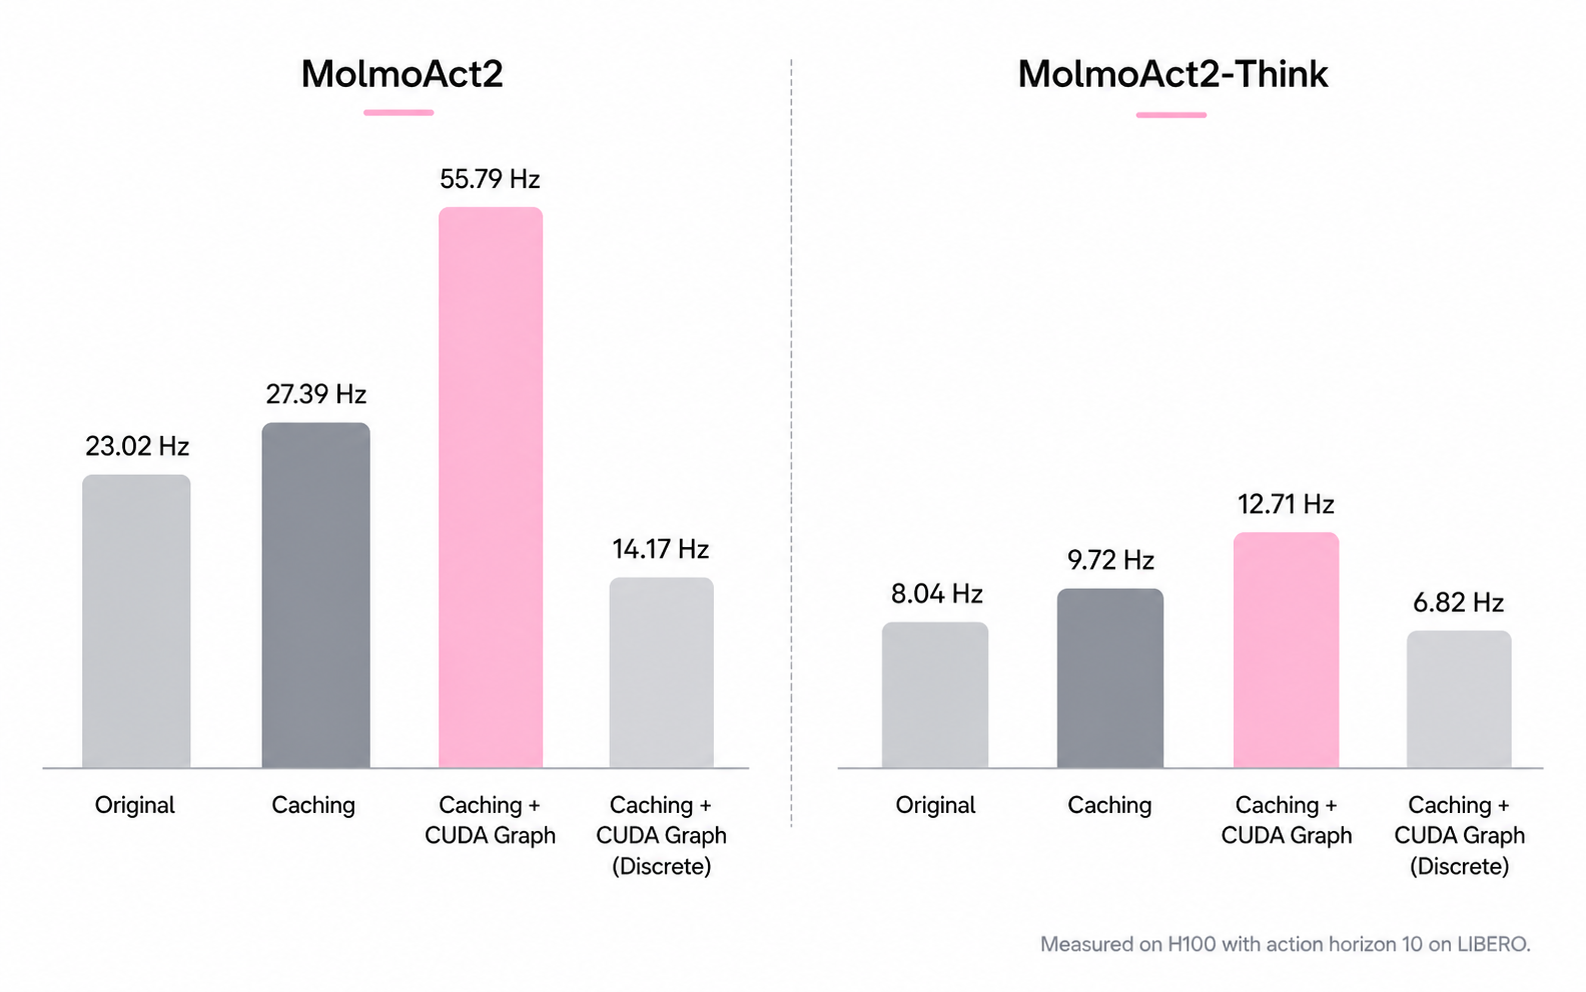
\includegraphics[width=0.7\linewidth]{figures/example_plot.png}
    \caption{\textbf{Single figure.} Replace \texttt{figures/example\_plot.png}
    with your own image. Use \texttt{width=...\textbackslash linewidth} to scale
    relative to the text width.}
    \label{fig:overview}
\end{figure}

\subsection{Component Two}
\label{subsec:component-two}
Explain the second component and how it connects to the first. Use
\texttt{subcaption} for multi-panel figures; reference a panel with
\cref{fig:panel-a} or the whole figure with \cref{fig:panels}.

\begin{figure}[t]
    \centering
    \begin{subfigure}{0.48\linewidth}
        \centering
        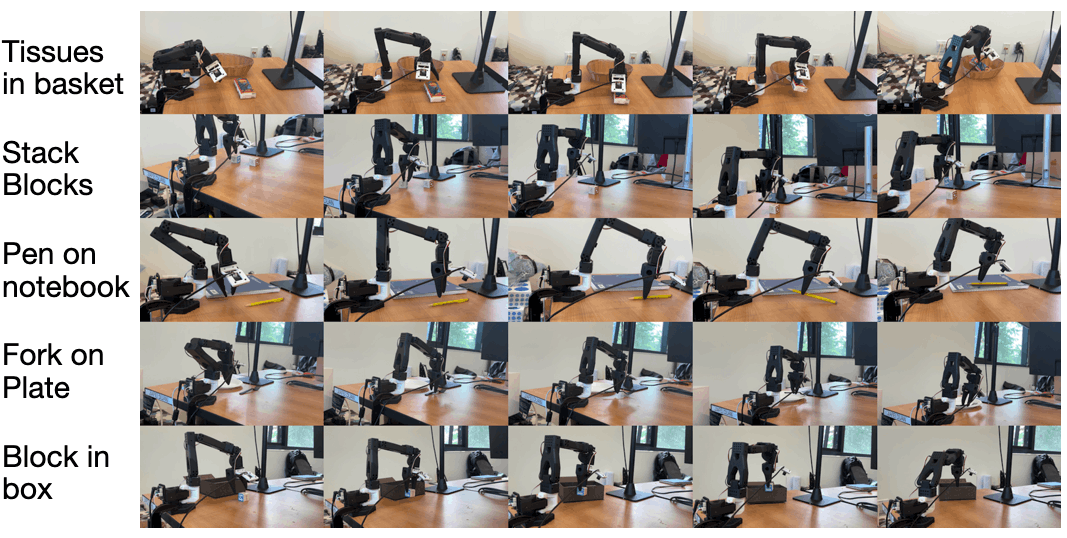
\includegraphics[width=\linewidth]{figures/example_panel_a.png}
        \caption{First panel.}
        \label{fig:panel-a}
    \end{subfigure}
    \hfill
    \begin{subfigure}{0.48\linewidth}
        \centering
        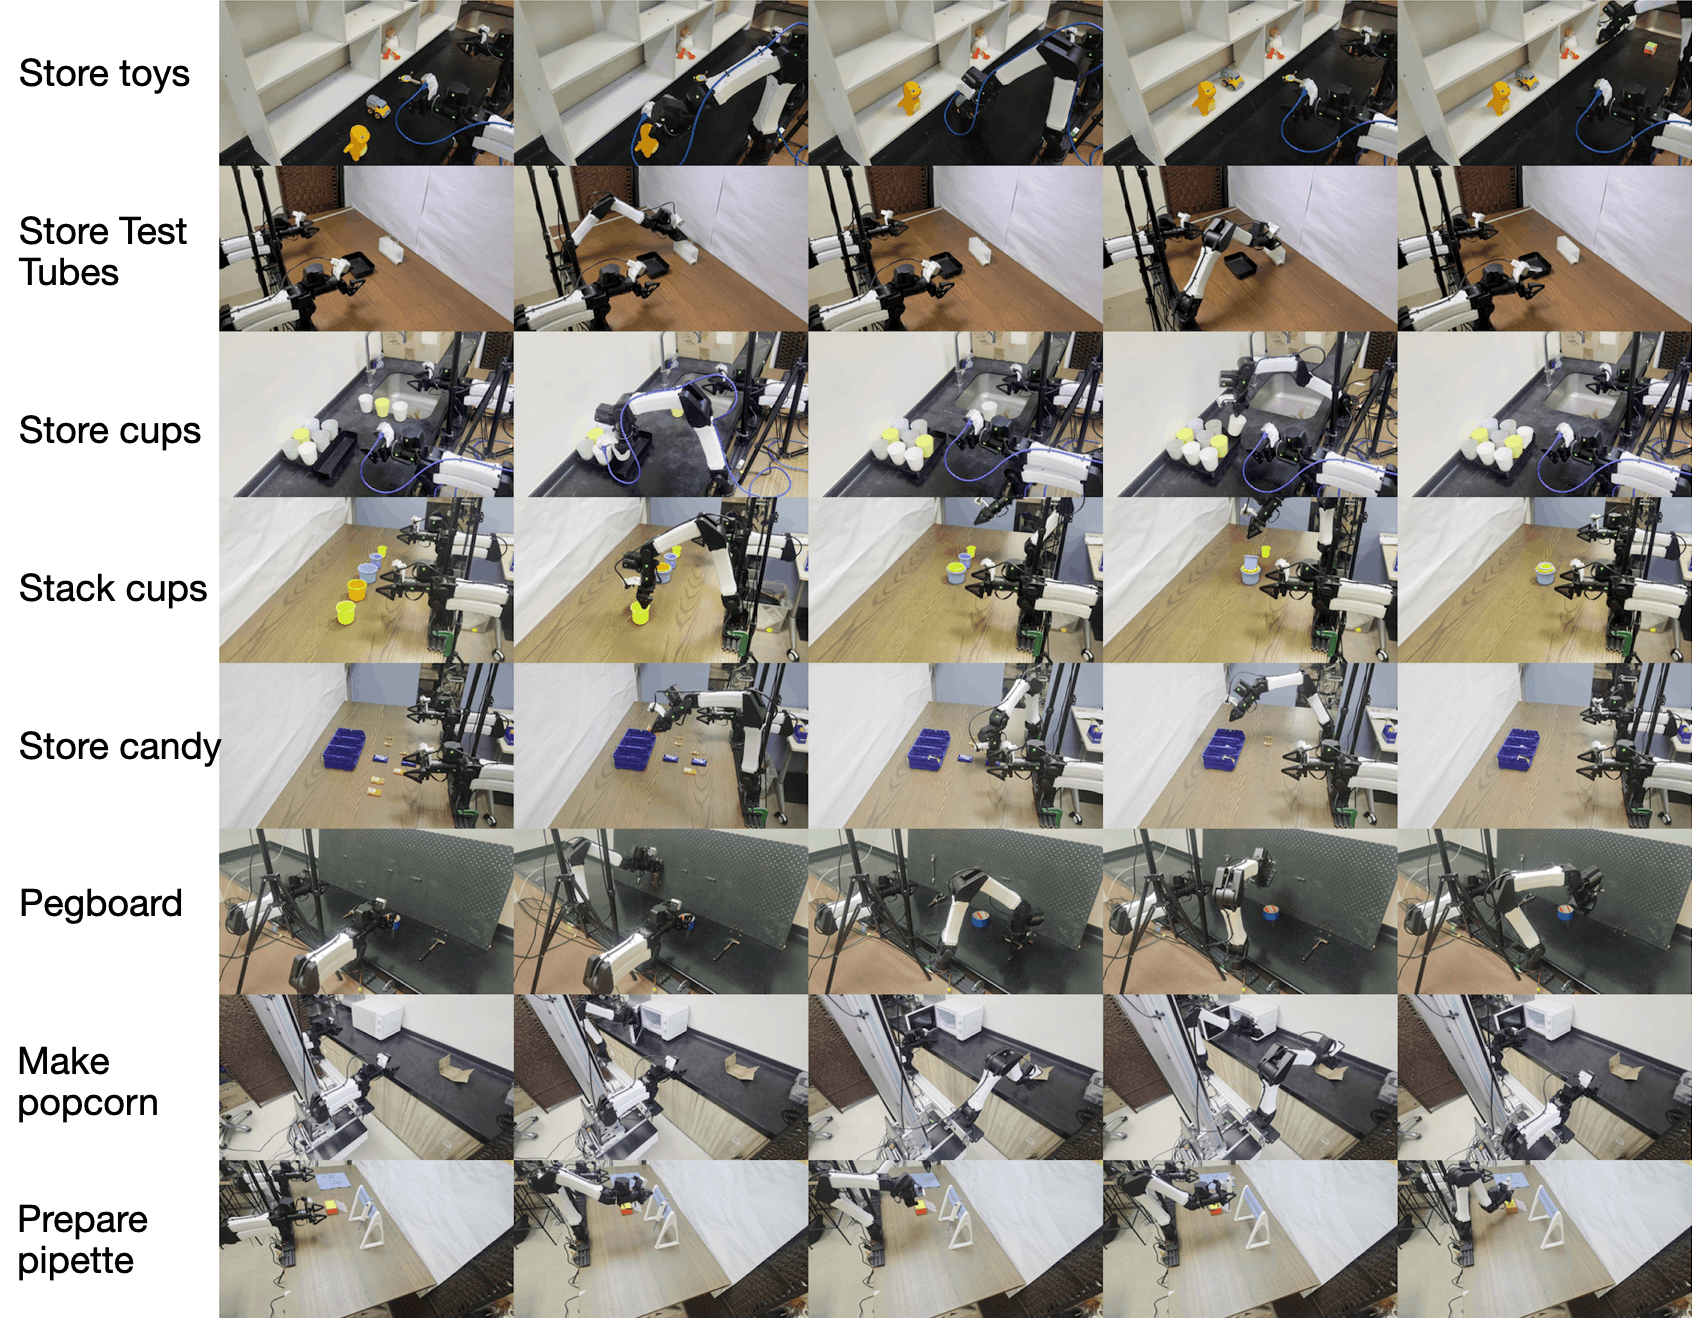
\includegraphics[width=\linewidth]{figures/example_panel_b.png}
        \caption{Second panel.}
        \label{fig:panel-b}
    \end{subfigure}
    \caption{\textbf{Two-panel figure.} Side-by-side images via the
    \texttt{subfigure} environment, each with its own sub-caption and label.}
    \label{fig:panels}
\end{figure}

